%% ****** Start of file apstemplate.tex ****** %
%%
%%
%%   This file is part of the APS files in the REVTeX 4 distribution.
%%   Version 4.1r of REVTeX, August 2010
%%
%%
%%   Copyright (c) 2001, 2009, 2010 The American Physical Society.
%%
%%   See the REVTeX 4 README file for restrictions and more information.
%%
%
% This is a template for producing manuscripts for use with REVTEX 4.0
% Copy this file to another name and then work on that file.
% That way, you always have this original template file to use.
%
% Group addresses by affiliation; use superscriptaddress for long
% author lists, or if there are many overlapping affiliations.
% For Phys. Rev. appearance, change preprint to twocolumn.
% Choose pra, prb, prc, prd, pre, prl, prstab, prstper, or rmp for journal
%  Add 'draft' option to mark overfull boxes with black boxes
%  Add 'showpacs' option to make PACS codes appear
%  Add 'showkeys' option to make keywords appear
\documentclass[aps,prl,twocolumn,superscriptaddress,floatfix]{revtex4-1}
%\documentclass[aps,prl,preprint,superscriptaddress]{revtex4-1}
%\documentclass[aps,prl,reprint,groupedaddress]{revtex4-1}

% You should use BibTeX and apsrev.bst for references
% Choosing a journal automatically selects the correct APS
% BibTeX style file (bst file), so only uncomment the line
% below if necessary.

\usepackage{graphicx}
\usepackage[caption=false]{subfig}
\usepackage{braket}
\usepackage{mathtools}
\usepackage{color}
\graphicspath{{figures/}}
\DeclareMathOperator{\sinc}{sinc}

\begin{document}

% Use the \preprint command to place your local institutional report
% number in the upper righthand corner of the title page in preprint mode.
% Multiple \preprint commands are allowed.
% Use the 'preprintnumbers' class option to override journal defaults
% to display numbers if necessary
%\preprint{}

%Title of paper
\title{Amplitude sensing with a trapped-ion mechanical oscillator}

% repeat the \author .. \affiliation  etc. as needed
% \email, \thanks, \homepage, \altaffiliation all apply to the current
% author. Explanatory text should go in the []'s, actual e-mail
% address or url should go in the {}'s for \email and \homepage.
% Please use the appropriate macro foreach each type of information

% \affiliation command applies to all authors since the last
% \affiliation command. The \affiliation command should follow the
% other information
% \affiliation can be followed by \email, \homepage, \thanks as well.
\author{K. A. Gilmore}
\email[]{kevin.gilmore@colorado.edu}
%\homepage[]{Your web page}
%\thanks{}
%\altaffiliation{}
\affiliation{National Institute of Standards and Technology, Boulder, Colorado 80305, USA}
\affiliation{JILA and Department of Physics, University of Colorado, Boulder, Colorado, 80309, USA}

\author{J. G. Bohnet}
\affiliation{National Institute of Standards and Technology, Boulder, Colorado 80305, USA}

\author{B. C. Sawyer}
\affiliation{Georgia Tech Research Institute, Atlanta, Georgia 30332, USA}

\author{J. W. Britton}
\affiliation{U.S. Army Research Laboratory, Adelphi, Maryland 20783, USA}

\author{J. J. Bollinger}
\affiliation{National Institute of Standards and Technology, Boulder, Colorado 80305, USA}

%Collaboration name if desired (requires use of superscriptaddress
%option in \documentclass). \noaffiliation is required (may also be
%used with the \author command).
%\collaboration can be followed by \email, \homepage, \thanks as well.
%\collaboration{}
%\noaffiliation

\date{\today}

\begin{abstract}
We present experimental and theoretical results demonstrating sensing of displacement amplitudes of our trapped-ion mechanical oscillator of 50 pm, 2 orders of magnitude smaller than the ground state wavefunction size. Our system is a 2-D array of Be+ ions in a Penning trap whose valence electron spins are coupled via a spin-dependent optical dipole force to the motional state of the ions. By reading out the dephasing of the spins, we are able to detect small displacements of the ion crystal. We document excellent theoretical agreement for the lineshapes, signal sizes, and sensitivity of our experiment. We perform these measurements off-resonantly and phase incoherently, but with near-term improvements expect to detect on-resonance sub-yN forces.
\end{abstract}

% insert suggested PACS numbers in braces on next line
\pacs{}
% insert suggested keywords - APS authors don't need to do this
%\keywords{}

%\maketitle must follow title, authors, abstract, \pacs, and \keywords
\maketitle

% If in two-column mode, this environment will change to single-column
% format so that long equations can be displayed. Use
% sparingly.
%\begin{widetext}
% put long equation here
%\end{widetext}

% figures should be put into the text as floats.
% Use the graphics or graphicx packages (distributed with LaTeX2e)
% and the \includegraphics macro defined in those packages.
% See the LaTeX Graphics Companion by Michel Goosens, Sebastian Rahtz,
% and Frank Mittelbach for instance.
%
% Here is an example of the general form of a figure:
% Fill in the caption in the braces of the \caption{} command. Put the label
% that you will use with \ref{} command in the braces of the \label{} command.
% Use the figure* environment if the figure should span across the
% entire page. There is no need to do explicit centering.

% \begin{figure}
% \includegraphics{}%
% \caption{\label{}}
% \end{figure}

% Surround figure environment with turnpage environment for landscape
% figure
% \begin{turnpage}
% \begin{figure}
% \includegraphics{}%
% \caption{\label{}}
% \end{figure}
% \end{turnpage}

% tables should appear as floats within the text
%
% Here is an example of the general form of a table:
% Fill in the caption in the braces of the \caption{} command. Put the label
% that you will use with \ref{} command in the braces of the \label{} command.
% Insert the column specifiers (l, r, c, d, etc.) in the empty braces of the
% \begin{tabular}{} command.
% The ruledtabular enviroment adds doubled rules to table and sets a
% reasonable default table settings.
% Use the table* environment to get a full-width table in two-column
% Add \usepackage{longtable} and the longtable (or longtable*}
% environment for nicely formatted long tables. Or use the the [H]
% placement option to break a long table (with less control than 
% in longtable).
% \begin{table}%[H] add [H] placement to break table across pages
% \caption{\label{}}
% \begin{ruledtabular}
% \begin{tabular}{}
% Lines of table here ending with \\
% \end{tabular}
% \end{ruledtabular}
% \end{table}

% Surround table environment with turnpage environment for landscape
% table
% \begin{turnpage}
% \begin{table}
% \caption{\label{}}
% \begin{ruledtabular}
% \begin{tabular}{}
% \end{tabular}
% \end{ruledtabular}
% \end{table}
% \end{turnpage}


% body of paper here - Use proper section commands
% References should be done using the \cite, \ref, and \label commands
% Put \label in argument of \section for cross-referencing
%\section{\label{}}
Measuring the amplitude of mechanical oscillators has engaged physicists for more than 50 years \citep{Weber1966} and, as the limits of amplitude sensing have dramatically improved, produced exciting advances both in fundamental physics and in applied work.  Examples include the detection of gravitational waves \citep{Abbott2016}, the coherent quantum control of mesoscopic objects \citep{Aspelmeyer2014}, improved force microscopy \citep{Butt2005}, and the transduction of quantum signals \citep{Palomaki2013}. During the past decade, optical-mechanical systems have demonstrated increasingly sensitive techniques for reading out the amplitude of a mechanical oscillator, with a recent demonstration obtaining a precision more than two orders of magnitude below the size of the ground state wave function (i.e. the amplitude of the zero-point fluctuations) \citep{Wilson2014a}. While optomechanical systems have assumed a wide range of physical systems, including toroidal resonators, nanobeams, membranes and others, the basic principle involves coupling the amplitude of a mechanical oscillator to the resonant frequency of an optical cavity mode \citep{Aspelmeyer2014}.

Crystals of laser-cooled, trapped ions behave as atomic-scale mechanical oscillators \citep{Jost2009,Biercuk2010,Sawyer2012} with tunable oscillator modes and high quality factors ($ > 10^4$) . Furthermore, the techniques of laser cooling enable ground state cooling of these oscillators. Trapped-ion crystals therefore provide an ideal experimental platform for investigating the fundamental limits of amplitude sensing, but to date there have only been a handful of investigations \citep{Biercuk2010,Sawyer2012,Shaniv2016,Knunz2010}. These investigations demonstrate amplitude detection comparable to or larger than the zero-point fluctuations of the trapped-ion oscillator.

In this Letter we experimentally and theoretically analyze a technique with which the center-of-mass (COM) motion of a 2-dimensional, trapped-ion crystal of $\sim$100 ions can be detected with a sensitivity several orders of magnitude below the zero-point fluctuations. Instead of coupling the motion to an optical mode of a cavity, we employ a time-varying spin-dependent force that couples the amplitude of the COM motion with internal spin degrees of freedom of the ions \citep{Sawyer2014,Ivanov2016}. When the frequency $\mu$ of the spin-dependent force matches the frequency $\omega$ of an imposed COM oscillation, $Z_{c}\cos\left(\omega t\right)$, spin precession proportional to $Z_{c}$ occurs, which we read out with a precision imposed by spin projection noise \citep{Itano1993}. Analogous to the canonical optomechanical coupling, here the amplitude of the trapped-ion oscillator produces a shift in the frequency of the spin (or qubit) degree of freedom of the trapped ions.

To demonstrate the sensitivity of this technique in the absence of noise and excitations of the COM mode, we perform measurements where $\omega$ is far from resonance with the mechanical COM resonance frequency $\omega_{z}$ of the ion array. We demonstrate a sensitivity of $(100\:\mathrm{pm})^{2}/\sqrt{Hz}$ ??? and the detection of amplitudes $Z_{c}$ as small as 50 pm, almost two orders of magnitude below the $\sim$2 nm ground state wave function size. For our set-up a 50 pm amplitude at a frequency $\omega$ far from resonance corresponds to an electric field detection of 0.46 mV/m  or 73 yN/ion. These force and electric field sensitivities can be improved by the Q of the COM mode by probing near resonance with $\omega_z$.  Further improvements can be obtained using techniques such as spin-squeezing \citep{Bohnet2015} to reduce projection noise of the readout.

\iffalse
Orig intro:
Well controlled and understood quantum systems offer advantages over their classical counterparts and are finding uses in a variety of up-and-coming disciplines. Quantum information and quantum cryptography are chief among them, but the use of such a quantum mechanical system as a sensor may prove to be tremendously useful. Quantum metrology, where the sensing protocol is enhanced by entanglement, is the most direct way to improve a measurement's sensitivity beyond the classical limit. However, such methods remain relatively far from useful application. The use of a quantum system sensitive to a physical parameter, such as an electric or magnetic field, is of more immediate usefulness for sensitive measurements \citep{Degen2016}. Cavity-based optomechanical resonators have proven to be tremendously sensitive to a wide variety of physical parameters and are the most prominent example of a mesoscopic system used as a quantum sensor \citep{Clark2016,Kampel2016,Kim2016a,Schreppler2014a}. Single ion sensors make use of their long coherence times to make measurements and are the prime example of a single quantum object used as a sensor \citep{Shaniv2016,Ivanov2016a,Knunz2010}. Our 2-D crystal of ions in a Penning trap operates in a regime between these two paradigms.
 
What these different experimental setups have in common as sensors is that they all make use of a mechanical oscillator. An ion in an RF trap oscillates at the trap resonance frequency. A microfabricated resonator is an oscillating membrane. The ion crystal in an Penning trap behaves like both: the drumhead modes of the crystal oscillate like a membrane with the center of mass mode at the trap resonance frequency. The sensing of an applied drive is done by measuring the displacement of the oscillator. Naturally, the best force sensitivity for such a mechanical oscillator occurs when the applied force is driven at the resonance frequency. Driving the oscillator with a small, off-resonant force requires greater displacement sensitivity - as the same force applied on resonance results in a much larger displacement. In addition, the standard quantum limit (SQL) and fundamental quantum limit (QL) converge at the resonance, but off-resonance the SQL may be surpassed \citep{Ivanov2016,Kampel2016,Schreppler2014a}. By operating off-resonantly, we can demonstrate in the future with phase-coherent detection amplitude sensing below the SQL.

By scaling up the number of ions we see an increase in sensitivity to ion displacement and electric fields compared to a single ion. Though our experiments are performed phase-incoherently and off-resonantly, with near-term improvements we expect to operate phase-coherently and on resonance with the center of mass mode frequency of the ion crystal. This would enable us to make use of recently demonstrated spin-squeezing in our ensemble of 100s of ions to perform further quantum enhanced sensing \citep{Bohnet2015}. As it stands, we are able to detect a displacement of 200 pm due to an RF drive applied to the trap endcap electrode. The ground state wavefunction size is 10 nm, 50 times as large.

We present a novel technique for amplitude and force sensing. By isolating and controlling a two-level system comprised of the effective spin-1/2 in each ion in our trap and applying a global spin-dependent force, the spin and motional degrees of freedom of the ions are coupled. This coupling allows us to measure the motional state of the ions by directly reading out the spin state. This method was used previously as a probe of the mode temperatures in the ion crystal in our Penning trap \citep{Sawyer2014a}.

A prior version of this experimental apparatus using Doppler velocimetry reported force sensing of 390 yN $Hz^{-1}$ and displacements of 18 nm \citep{Biercuk2010a, Biercuk2011}. With near term improvements we expect to best this force sensitivity by []. We report an amplitude sensitivity two orders of magnitude improved.
\fi
\begin{figure}
    \centering
    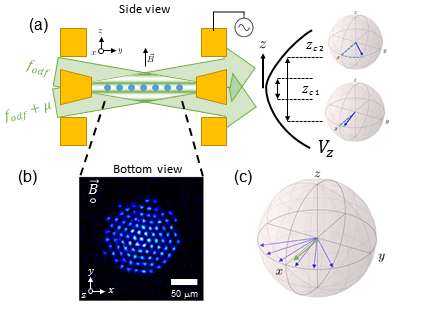
\includegraphics[width=.5\textwidth]{expt3}
    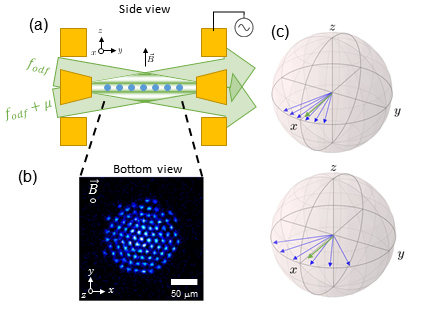
\includegraphics[width=.5\textwidth]{expt4}
    \caption{(a) Cross-section of the NIST Penning trap, characterized by an axial magnetic field $B = 4.45$ T and an axial trap frequency $\omega_z = 2\pi \times 1.57$ MHz. The blue dots represent the ions. Cylindrical electrodes (yellow) generate a harmonic confining potential along their axis. Radial confinement is provided by the Lorentz force from $\vec{E} \times \vec{B}$-induced rotation in the axial magnetic field. Time varying potentials applied to eight azimuthally segmented electrodes generate a rotating wall potential that controls the crystal rotation frequency. Doppler cooling beams are directed along $y$ and $z$. The beams generating the spin-dependent optical dipole force cross the ion plane at $\pm 10^{\circ}$, forming a 1-dimensional optical lattice (green lines) with a 0.9 $\mu$m wavelength. Global, state-dependent fluoresence is collected on the side-view objective. (b) Bottom-view image of ion crystal. (c) Dephasing of the spins after rotation to the equator of the Bloch sphere. }
    \label{Expt}
\end{figure}
Our experimental apparatus, described in Fig. \ref{Expt} and \citep{Sawyer2014,Bohnet2015}, consists of $N\sim100$ $\prescript{9}{}{}$Be$^{+}$ ions laser-cooled to the Doppler limit of 0.5 mK and confined to a single-plane Coulomb crystal in a Penning trap. The spin-1/2 or qubit degree of freedom is the $\prescript{2}{}{S}_{1/2}$ ground-state valence electron spin $\ket{\uparrow} (\ket{\downarrow}) \equiv \ket{m_{s}=+1/2} (\ket{m_{s}=-1/2}) $. In the magnetic field of the Penning trap, the ground state is split by 124 GHz. A resonant microwave source is used to perform global rotations of the spin ensemble. A pair of laser beams, detuned from any optical transitions by $\sim$20 GHz, interfere to form a 1-dimensional optical lattice, resulting in a spin-dependent optical dipole force (ODF) that couples the spins to the ions's axial motion. The cooling and repump transitions allow for efficient preparation of all N trapped ions to the state $\ket{\uparrow}_N \equiv \ket{\uparrow \uparrow \cdots \uparrow}$. At the end of the experiments described here we measure the average probability $P_\uparrow$ for an ion spin to be in $\ket{\uparrow}$ from a global measurement of state-dependent resonance fluorescence on the Doppler cooling transition. This is equivalent to measuring the z-component of the composite Bloch vector of the spins.
\iffalse
\begin{figure}[h]
  \subfloat[]{%
    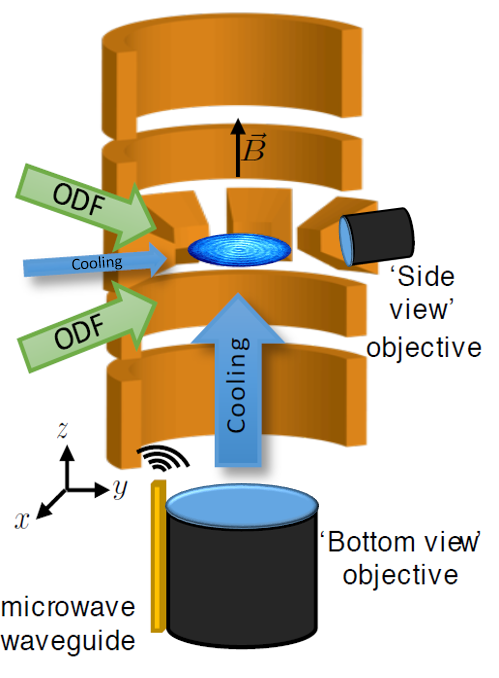
\includegraphics[width=.24\textwidth]{penning_trap}}\hfill
  \subfloat[]{%
    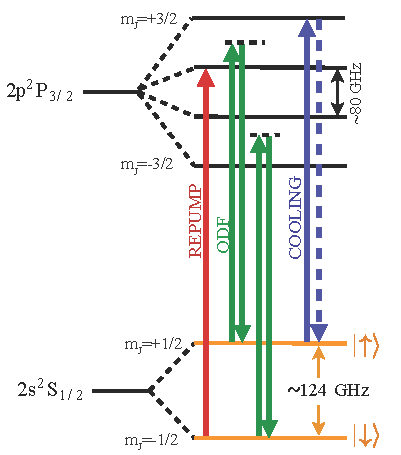
\includegraphics[width=.24\textwidth]{level_diagram}}\hfill
  \caption{(a) Cross-section of the NIST Penning trap, characterized by an axial magnetic field $B = 4.45$ T and an axial trap frequency $\omega_z = 2\pi \times 1.57$ MHz. The blue disk represents the ion crystal. Cylindrical electrodes (orange) generate a harmonic confining potential along their axis. Radial confinement is provided by the Lorentz force from $\vec{E} \times \vec{B}$-induced rotation in the axial magnetic field. Time varying potentials applied to eight azimuthally segmented electrodes generate a rotating wall potential that controls the crystal rotation frequency. Doppler cooling beams are directed along $y$ and $z$. The beams generating the spin-dependent optical dipole force cross the ion plane at $\pm 10^{\circ}$, forming a 1-dimensional optical lattice with a 0.9 $\mu$m wavelength. Global, state-dependent fluoresence is collected on the side-view objective. (b) Energy levels of $\prescript{9}{}{}$Be$^{+}$ at B = 4.46 T showing the different laser frequencies used to Doppler cool, optically pump, and couple the spin and motional degrees of freedom.}\label{Fig 1}
\end{figure}
\fi
%By measuring the decrease in the composite Bloch vector length produced %by the application of a homogenous spin-dependent force, detailed %information about the motional state of the ions is revealed. This spin %dephasing is directly measured. The spin-dependent optical dipole force %(ODF) is generated from the interference of a pair of detuned lasers, %shown in Fig. \ref{Fig 1} (a). 


The ODF couples the spin and motional degrees of freedom through the interaction [Bohnet Science supplementary]
\begin{equation}
H_{ODF} = U\sum_{i}\sin(\delta k \cdot \hat{z}_{i} - \mu t + \phi)\hat{\sigma}^{z}_{i} ,
\label{Hodf}
\end{equation}
where $\delta k$ is the wave vector describing the 1D optical lattice, $\mu$ ($\phi$) is the frequency (phase) difference between the ODF beams, and $\hat{z}_{i}$ and $\hat{\sigma}^{z}_{i}$ are the position operator and Pauli spin matrix for ion $i$. We work in a regime where Lamb-Dicke confinement is approximately satisfied, $\delta k \left< \hat{z}^{2}_{i} \right>^{1/2} \lesssim 0.5$. In this case, and assuming $U/\mu \ll 1$, Eq. \ref{Hodf} can be approximated as
\begin{equation}
H_{ODF} \approx  U\sum_{i}\sin(\delta k \cdot \hat{z}_{i})\cos(\mu t - \phi)\hat{\sigma}^{z}_{i}.
\label{Hodf_simple}
\end{equation}
With an rf tickle on one of the trap electrodes at a frequency $\omega$ far from any of the axial drumhead modes, we impose a weak, classically driven COM motion of constant amplitude and phase, $\hat{z}_i \rightarrow \hat{z}_i +Z_c\cos(\omega t+\delta)$.  With $\delta k Z_c \ll 1$ and assuming $\mu\sim\omega$,  Eq. \ref{Hodf_simple} can be simplified to describe the shift in the qubit transition frequency due to the coherent amplitude $Z_c$,
\[H_{ODF} = DWF \cdot U \cdot \delta k \cdot Z_c\cos((\omega - \mu)t + \delta + \phi) \sum_{i} \frac{\hat{\sigma}^{z}_{i}}{2} .\]
Here $DWF \equiv \exp(-\delta k^2 \left< \hat{z}^{2}_{i} \right> / 2) \approx 0.86 $ is the Debye-Waller factor, a reduction in interaction strength due to the departure from the Lamb-Dicke confinement regime \citep{Wineland1998a}.  

For $\mu = \omega$ there is a static shift $\Delta(Z_c)$ in the frequency of the qubit transition, 
\begin{equation}
\Delta(Z_c) = DWF \cdot (U/\hbar) \cdot \delta k \cdot Z_c \cos(\delta + \phi).
\label{frequency shift}
\end{equation}
For the moment, we assume $\delta+\phi=0$.  Then $\Delta(Z_c)$, the zero-point fluctuations of the COM mode for $N=100$ evaluated at $Z_c = \frac{1}{\sqrt{N}}\sqrt{\frac{\hbar}{2m\omega_z}}\approx 1.9$ nm, is the equivalent vacuum optomechanical coupling strength  $g_0$ \citep{Aspelmeyer2014} for our set-up. With  $\delta k =2\pi/900$ nm (see Fig. \ref{Expt}) and a modest 1D lattice potential $U/\hbar = 2\pi \times (10\:kHz)$, typical of that employed here, $\Delta(1.9\:nm) \approx 710\:s^{-1}$.  We measure $\Delta(Z_c)$ from the resulting spin precession in a Ramsey-style experiment like that discussed in Fig. \ref{Fig Ramsey}. If $\tau$ is the total ODF interaction time of the sequence, the resulting spin precession on resonance $(\mu = \omega)$ is simply $\theta = \theta_{max} \cos(\delta+\phi)$ where $\theta_{max} \equiv DWF \cdot (U/\hbar) \cdot \delta k\;Z_c \cdot \tau$.


%some original text here:
%Tuning the ODF difference frequency allows for readout of the motional state of the ions at that frequency by measuring the precession of the spins about the Bloch sphere and, in a typical Ramsey style experiment, projecting this on to the dark state (spin-down). Spin-dephasing, then, appears as an increase in spin-up population. The precession due to an axial oscillation can be determined by considering a classical driven motion of constant amplitude $z_{0}$, frequency $\omega$, and phase $\delta$, $z_i \rightarrow z_i +z_0\cos(\omega t+\delta)$.
%Then,
%\[H_{ODF} = DWF \cdot U \cdot \delta k \cdot z_0\cos((\omega - \mu)t + \delta + \phi) \sum_{i} \frac{\sigma^{z}_{i}}{2} \]
%where $DWF = \exp(-\delta k^2 \left< z^{2}_{i} \right> / 2) $ is the Debye-Waller factor, a reduction in interaction strength as a function of departure from the Lamb-Dicke regime.
%For the case $ \omega = \mu $, where the ODF frequency difference is equal to the frequency of the applied drive,
%\[\theta = \Delta\tau = DWF \cdot U \cdot \delta k \cdot z_0 \cdot \tau \cos(\delta - \phi) = \theta_{max}\cos(\delta - \phi)\]
%where $\Delta$ is the energy difference between spin-up and spin-down for each ion and $\tau$ is the total ODF interaction time. $\theta_{max}$ is the maximum precession, which occurs when the drive is in phase with the ODF beatnote.
%\begin{figure}[h]
%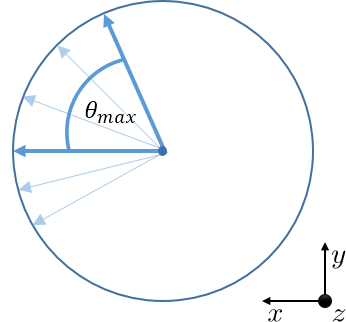
\includegraphics[width=.15\textwidth]{dephasing}
%\caption{After rotating to the equator on the Bloch sphere, an incoherent axial perturbation causes precession. The maximum precessed angle is $\theta_{max}$.}\label{Fig 2}
%\end{figure}

Due to phase instabilities in our current implementation of the ODF interaction, we measure the induced spin precession phase incoherently. If the phase of the applied force was unknown or time-dependent, this phase-incoherent sensing would be necessary - and so, our experiment represents a `worst-case' sensing experiment. In the phase-incoherent picture, the relative phase between the drive ($\delta$) and the ODF beat note ($\phi$) is sampled randomly with each repetition of the experiment. Different experimental trials therefore result in a different precession $\theta = \theta_{max} \cos(\phi+\delta)$. We measure the decrease (or decoherence) in the average length of the Bloch vector resulting from this random precession. In a Ramsey sequence where a Bloch vector undergoing no precession is rotated to the dark state $\ket{\downarrow}_N$ (see Fig. \ref{Fig Ramsey}), the average probability for measuring spin-up is $\left< P_{\uparrow} \right> = \frac{1}{2}[1-e^{-\Gamma \tau} \left<\cos(\theta)\right>]$. Here $\Gamma = \frac{1}{2}(\Gamma_{el} + \Gamma_{ram})$ is the decay rate from spontaneous emission from the off-resonant ODF laser beams, where $\Gamma_{el}$ ($\Gamma_{ram}$) is the elastic (Raman) scattering decoherence rate \citep{Uys2010}. The average $ \left< \cos(\theta) \right> $ is over the random phase $\phi+\delta$ with the result $ \left< \cos(\theta) \right> = J_0(\theta_{max}) $, where $J_0$ is the zeroth order Bessel function of the first kind. Thus,
\begin{equation}
\left< P_{\uparrow} \right> = \frac{1}{2} \left[ 1-e^{-\Gamma \tau}J_0(\theta_{max}) \right].
\label{Bessel}
\end{equation}
We note that the incoherent sensing described by Eq. \ref{Bessel} is second-order sensitive to $\theta_{max}$ (or $Z_c$).

To create the steady-state COM axial oscillation $Z_c \cos(\omega t+\delta)$, we applied a continuous AC voltage (i.e. an rf tickle) to an endcap of the Penning trap at a frequency near $\omega/(2\pi) = 400$ kHz. This frequency was chosen because it was far from any mode frequencies of the array, and there were no observed sources of noise. Specifically application of the ODF interaction with $\mu/(2\pi) \approx 400$ kHz and no rf tickle resulted in a background given by Eq. \ref{Bessel} with $\theta_{max}=0$. Characterization of the detection sensitivity requires calibration of the applied AC voltage in terms of ion displacement. We calibrated the displacement of the ions due to a static voltage applied to the endcap by measuring the resulting movement of the ion crystal in the side-view imaging system. From this calibration, we determine that a 1 V offset results in a 0.97 $\pm$ 0.009 $\mu$m displacement of the ions. We estimate that the corrections for using this DC calibration with an $\omega/(2\pi) \approx 400$ kHz drive is less than 10$\%$. 


%To create an axial oscillation, we apply an AC voltage to the endcap of the Penning trap. This can be done either on-resonance or off-resonance with the center of mass mode of the ion crystal at $2\pi \times 1.57$ MHz. Characterization of the detection sensitivity requires calibration of the applied drive in terms of ion displacement. To calibrate the displacement of the ions as a result of this applied drive, we apply a static voltage to the endcap and measure the deflection of the ion crystal. The deflection is measured using an f/10 light collection system and a CCD camera, which provides spatial resolution of $\sim .8 \mu$m per pixel. From this calibration, we find 1 V results in 0.97 $\pm$ 0.009 $\mu$m of displacement.

%Away from its resonance frequency the driven motion of a mechanical oscillator is damped and its sensitivity to an applied force is lessened. Motivated by investigating low frequency noise sources in our laboratory and by demonstrating sensitivity to small displacements, we performed our experiments far from the center-of-mass mode frequency of our ion crystal. By applying a $\sim$400 kHz drive to the endcap electrode, we can study the response of the ion harmonic oscillator to an off resonant force. For this paper, we are interested in presenting the ultimate off-resonance amplitude sensitivity of our apparatus.

Our experimental sequence makes use of the quantum lock-in technique wherein the phase accumulated due to spin-precession in each arm of the sequence is added coherently \citep{Kotler2011}. To decouple from magnetic field fluctuations over the course of the experiment, a spin echo style sequence is used. Figure 2 shows a CPMG sequence - a multipulse extension of the Hahn spin echo - with two $\pi$ pulses and phase jumps appropriate for adding the phases. The general experimental sequence is as follows. A calibrated drive at $\sim$400 kHz is applied to the endcap of the trap and left on throughout the experiment. The ions are prepared in $\ket{\uparrow}_N$ with cooling and repump lasers. A microwave $\pi/2$ pulse rotates the spins to the $\hat{x}$ axis, to the superposition $\left[\ket{\uparrow} + \ket{\downarrow}\right]/\sqrt{2}$. The ODF beams are pulsed on for a duration T followed by a microwave $\pi$ pulse about $\hat{x}$ and another ODF pulse of duration T. This ODF-$\pi$-ODF sequence is repeated $n$ times. After a second $\pi/2$ pulse about $\hat{y}$, the final state readout measures the population of the spins in $\ket{\uparrow}$ via global fluorescence due to photons scattered from the cooling beam. Using $n = 8$ ODF-$\pi$-ODF pulses allows us to push the sequence time out to 20 ms and maintain a background fully characterized by decoherence due to spontaneous emission. This sequence, with fixed ODF evolution times T, is sensitive to particular modulation frequencies given by $ \omega/2\pi = (2n+1)/(2(T+t_{\pi}))$. In principle, given a signal with a certain frequency T would be adjusted accordingly.
\iffalse
\begin{figure*}[h]
  \subfloat[]{%
    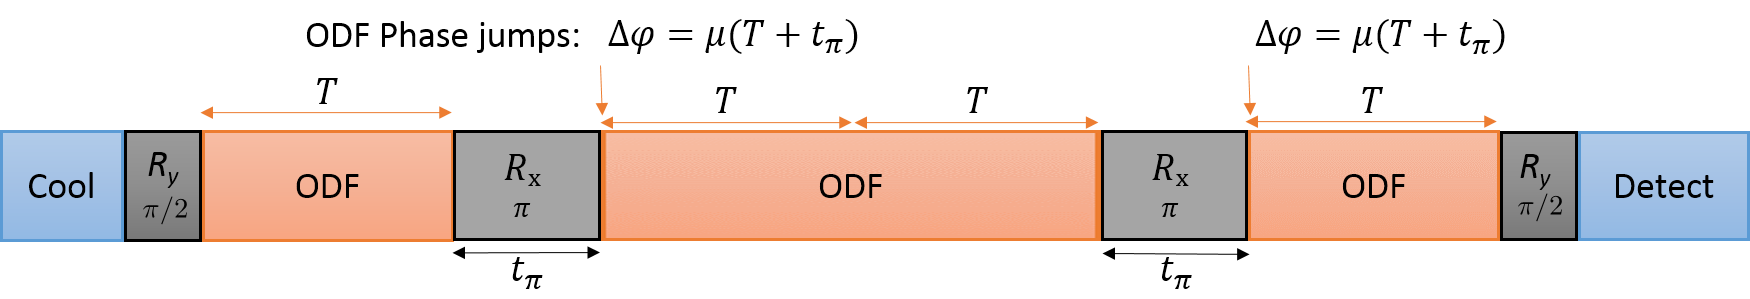
\includegraphics[width=.8\textwidth]{cpmg}}\\
  \subfloat[]{%
    
\includegraphics[width=.8\textwidth]{8pi_cpmg}}\\
  \subfloat[]{%
    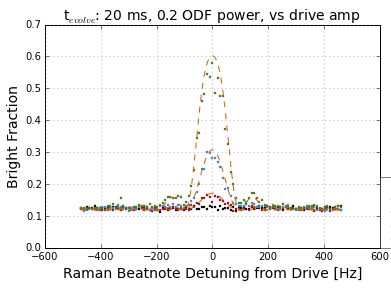
\includegraphics[width=.45\textwidth]{lineshape_vs_drive}}\hfill
  \subfloat[]{%
    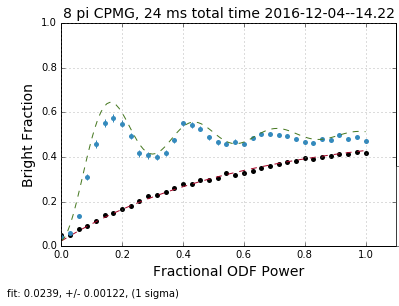
\includegraphics[width=.45\textwidth]{pwr_scan}}
  \caption{(a) CPMG sequence with two $\pi$ pulses. Orange blocks represent ODF pulses, grey microwave rotations, and blue cooling and detecting. In this experiment, the classical drive is left on throughout. After each $\pi$ pulse, the ODF phase is jumped in order to sum the phases accumulated in each ODF arm. The phase jump $\Delta\varphi = \mu(T+t_{\pi})$ is chosen to cancel a term in the Hamiltonian relevant at low frequencies $\mu$ (when the approximation  $U/\mu \ll 1$ does not hold) so that Eq. 2 remains valid. (b) CPMG sequence with 8 $\pi$ pulses. Cooling and detection remain the same, and the phase is jumped by the same amount after each $\pi$ pulse. Chaining the ODF pulses in this fashion allows us to go to much longer total interaction times (20 ms) and detect smaller displacements. (c) Lineshape of the classical drive for drive amplitudes of 500 pm (red), 1 nm (blue) and 2 nm (green). Black points are background, with drive turned off. Dashed lines are theory curves with no free parameters.  (d) Lineshape for classical drive displacement of 500 pm and  fractional ODF power of 1 (red), 0.5 (green), 0.3 (purple), and 0.15 (dark green). As the ODF power is increased, the background rises and the optimal signal-to-noise is found.}\label{Fig Ramsey}
\end{figure*}
\fi
\begin{figure*}
    \centering
    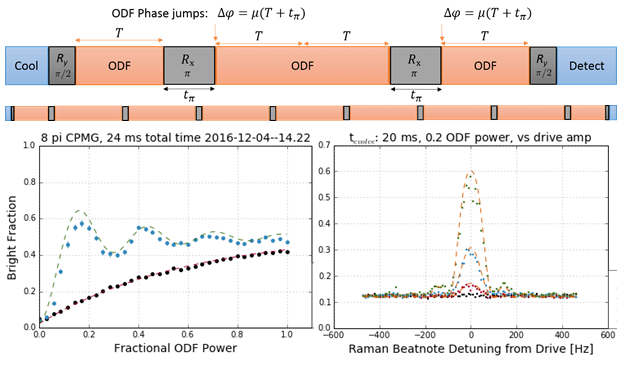
\includegraphics[width=.8\textwidth]{amp_sensing}
  \caption{(a) CPMG sequence with two $\pi$ pulses. Orange blocks represent ODF pulses, grey microwave rotations, and blue cooling and detecting. In this experiment, the classical drive is left on throughout. After each $\pi$ pulse, the ODF phase is jumped in order to sum the phases accumulated in each ODF arm. The phase jump $\Delta\varphi = \mu(T+t_{\pi})$ is chosen to cancel a term in the Hamiltonian relevant at low frequencies $\mu$ (when the approximation  $U/\mu \ll 1$ does not hold) so that Eq. 2 remains valid. (b) CPMG sequence with 8 $\pi$ pulses. Cooling and detection remain the same, and the phase is jumped by the same amount after each $\pi$ pulse. Chaining the ODF pulses in this fashion allows us to go to much longer total interaction times (20 ms) and detect smaller displacements. (c) As a function of measurement strenght (ODF power), the background (black points) with no applied drive and signal (blue points) for a 2.5 nm displacement is shown. The red curve is a fit to the background. The green curve is the theoretical prediction given the background with no free parameters. The oscillations are due to the Bessel function behavior of the signal. (d)Lineshape of the classical drive for drive amplitudes of 500 pm (red), 1 nm (blue) and 2 nm (green). Black points are background, with drive turned off. Dashed lines are theory curves with no free parameters.}\label{Fig Ramsey}
\end{figure*}
To model the lineshape of the signal, it is necessary to account for the accumulated phase due to the spin-dependent ODF potential without making the simplification that $ \omega = \mu $. This results in a characteristic response function for each sequence. For the $n = 8$ CPMG sequence the response function is given by:
%\begin{widetext}
%\begin{equation}
%\theta_{tot} = \theta_{max} \left[ \frac{2 \sin(\frac{1}{2}[(\omega-\mu)T])}{\omega-\mu} \right] 
%\left[ \sin(\frac{\omega}{2}(T+t_{\pi})) \right] \left[ \sin(\frac{1}{2}[\omega (T+t_{\pi}) + (\omega - \mu)T)]) \right] \left[ \cos(\omega(T+t_{\pi})+(\omega - \mu)T) \right] \left[ \cos(2(\omega(T+t_{\pi})+(\omega - \mu)T)) \right] 
%\end{equation}
%\end{widetext}

\begin{widetext}
\begin{equation}
\theta_{tot} = \theta_{max} \left[ \sinc \left( \frac{T}{2} \left( \omega-\mu \right) \right) \right] 
\left[ \cos \left( \frac{T}{2} \left( \omega - \mu \right) \right) \right] \left[ \cos(T(\omega - \mu)) \right] \left[ \cos(2T(\omega - \mu)) \right] .
\end{equation}
\end{widetext}

\begin{widetext}
\begin{equation}
\theta = \frac{DWF \cdot (U/\hbar) \cdot \delta k\;Z_c}{2}  \sinc\left( \frac{T}{2} \left( \omega-\mu \right) \right) \sin\left( \frac{\omega}{2} \left( T+t_{\pi} \right) \right) \sin(\xi)\cos(2 \xi)\cos(4 \xi),
\end{equation}
\end{widetext}

where $\xi = \frac{1}{2}\left( T(\omega - \mu) + \omega(T+t_{\pi}) \right)$. Figure \ref{Fig Ramsey} (c) shows the emergence of the signal out of the background as the drive amplitude is increased. Figure \ref{Fig Ramsey} (d) shows the evolution of the signal relative to the background as the power of the ODF beams is increased. In both cases the theory has no free parameters. The background is accounted for by independent measurements of spontaneous emission. The spontaneous emission decay rates are calculated from the measured AC Stark shifts induced by each ODF laser beam, a proxy for the laser intensity at the ions.

With the drive frequency chosen to correspond to the signal peak, scanning the power of the ODF laser varies the strength of the measurement. By comparing the curve to the background for particular drive amplitudes, the signal and the signal-to-noise can be extracted. From this, the sensitivity of the sequence is found. To calculate the signal-to-noise ratio, a value for $\theta^{2}_{max}$ needs to be extracted. Solving for $J_0(\theta_{max})$ given $\left< P_{\uparrow} \right>$ with the classical drive applied and $\left< P_{\uparrow} \right>_{bck}$ with no drive yields
\begin{equation}
J_0(\theta_{max}) = \frac{1-2\left< P_{\uparrow} \right>}{1-2\left< P_{\uparrow} \right>_{bck}}.
\end{equation}

The signal-to-noise for a single experiment is given by $S/N =\theta_{max}^{2}/\delta \theta_{max}^{2}$, where $\delta \theta_{max}^{2} \equiv \delta F(\theta_{max}^{2})/ \left( \frac{dF(\theta_{max}^{2})}{d\theta_{max}^{2}} \right)$ and  $F(\theta_{max}^{2}) \equiv \frac{1-J_0(\theta_{max})}{2}$. Then $\delta J_0(\theta_{max}) = 2e^{\Gamma \tau} \sqrt{\sigma^{2}_{P_{\uparrow}} + \delta \left< P_{\uparrow} \right>^{2} + \delta\left< P_{\uparrow} \right>^{2}_{bck}}$, where $\sigma^{2}_{P_{\uparrow}}$ is the variance due to shot-to-shot fluctuations of $\cos(\theta)$ caused by the incoherence between the phase of the applied drive and the ODF beatnote, $\delta \left< P_{\uparrow} \right>$ is the projection noise from the measurement of $P_{\uparrow}$, and $\delta \left< P_{\uparrow} \right>_{bck}$ is the noise in the background. As the drive amplitude is decreased, the relative contribution of $\sigma^{2}_{P_{\uparrow}}$ to the noise decreases as well, and the projection noise becomes dominant. In this regime, the signal-to-noise ratio begins to drop, representing the limit of sensitivity for this experiment. To extract this limit, we plot the signal-to-noise as a function of ion displacement in Fig. \ref{Fig sens}. 

To explore the ultimate limits of sensitivity of our setup, we repeat the aforementioned experimental sequence first without the applied drive on - to get the background - and then with the drive. We calculate the experimental signal-to-noise as follows. For a particular applied drive with known calibrated ion displacement, the experimental sequence is repeated 3000 times. With the assumption that $\theta_{max}$ is small, 

\begin{equation}
\frac{\theta^{2}_{max}}{8} = \frac{P_{\uparrow} - P_{\uparrow bck}}{1-2\left< P_{\uparrow} \right>_{bck}},
\end{equation}
where the numerator is the difference between sequential experiments with and without the applied drive and $\left< P_{\uparrow} \right>_{bck}$ is the background averaged over the 3000 repetitions. Then the experimentally determined signal-to-noise is

\begin{equation}
\frac{S}{N} = \left< \frac{\theta^{2}_{max}}{\sigma(\theta^{2}_{max})} \right>,
\end{equation}
where $\sigma(\theta^{2}_{max})$ is the standard deviation of the experimentally determined values of $\theta^{2}_{max}$ and the brackets represent an average over all repetitions.
\begin{figure}
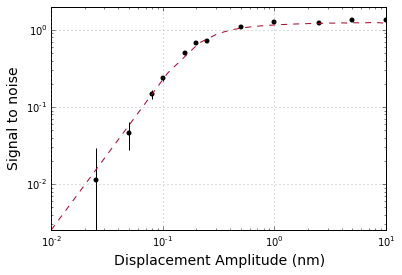
\includegraphics[width=.45\textwidth]{sense_lim}
\caption{Limit of amplitude sensing. As the amplitude of the applied drive is decreased, the projection noise of the spin ensemble dominates and the signal-to-noise ratio decreases. At larger amplitudes, the shot-to-shot fluctuations of the precession angle $\theta^{2}$ limit the signal-to-noise ratio to $\sim$ 1. Error bars represent the standard error.}\label{Fig sens}
\end{figure}

In summary, we have presented a novel technique for amplitude and force sensing. By isolating and controlling a two-level system comprised of the effective spin-1/2 in each ion in our Penning trap and applying a global spin-dependent force, the spin and motional degrees of freedom of the ions are coupled and the motional state of the ions may be directly read out from the spin state. We have documented, with excellent theoretical agreement, the response of our trapped-ion mechanical oscillator to an applied off-resonant drive and demonstrated a sensitivity of $(100\:\mathrm{pm})^{2}/\sqrt{Hz}$ ??? and the detection of amplitudes $Z_{c}$ as small as 50 pm, almost two orders of magnitude below the $\sim$2 nm ground state wave function size. Though our experiments are performed phase-incoherently and off-resonantly, with near-term improvements we expect to operate phase-coherently and on resonance with the center of mass mode frequency of the ion crystal. This would enable us to make use of recently demonstrated spin-squeezing in our ensemble of 100s of ions \citep{Bohnet2015} to perform further quantum enhanced sensing \citep{Ivanov2016}. When $\mu$ is applied on resonance with $\omega_{z}$, the force and electric field sensitivities can be improved by the Q of the COM mode, where we estimate Q$\sim10^{4}$ to $10^{5}$ for our set-up. Driving the oscillator with a small, off-resonant force requires greater displacement sensitivity - as the same force applied on resonance results in a much larger displacement. In addition, the standard quantum limit and fundamental quantum limit converge at the resonance, but off-resonance the SQL may be surpassed \citep{Ivanov2016,Kampel2016,Schreppler2014a}. Our trapped ion platform provides the control and sensitivity to investigate protocols that minimize back action. By operating off-resonantly, we can demonstrate in the future with phase-coherent detection amplitude sensing below the standard quantum limit.

% Specify following sections are appendices. Use \appendix* if there
% only one appendix.
%\appendix
%\section{}

% If you have acknowledgments, this puts in the proper section head.
%\begin{acknowledgments}
% put your acknowledgments here.
%\end{acknowledgments}

% Create the reference section using BibTeX:
\bibliographystyle{apsrev4-1}
%\bibliographystyle{apalike}

\bibliography{Force_sensing}

\end{document}
